
% ========================================================================== %
%                                                                            %
%                                 PREAMBLE                                   %
%                                                                            %
% ========================================================================== %

% Define document class
\documentclass[a4paper,11pt,titlepage]{article}
\usepackage[onehalfspacing]{setspace}

% Define geometry/positioning of of text
\usepackage[paper=a4paper,left=20mm,right=20mm,top=30mm,bottom =30mm]{geometry}

% Grammatic packages
\usepackage[ngerman,english]{babel}
\usepackage[utf8]{inputenc}
\usepackage[T1]{fontenc}
\usepackage[font=small, textfont=it, labelfont=it,bf, format=hang]{caption}

% Create headers
\usepackage{fancyhdr}
\pagestyle{fancy}
\headheight 14pt
\renewcommand{\headrulewidth}{0.4pt}
\renewcommand{\footrulewidth}{0.4pt}

% To comment text blocks
\usepackage{comment}  % --> \begin{comment} ... \end{comment}

% Packages affecting text, pictures and tables
\usepackage{multicol} 
\usepackage{graphicx}
\usepackage{caption}
\usepackage{float}
\usepackage{array}
\usepackage{booktabs}
\usepackage{xcolor}
\usepackage[section]{placeins} 	% pictures won't jump into other sections!
\usepackage{wrapfig} % Text aside pictures
\usepackage{rotating} % Allows rotated picturses AND captions!
\usepackage{pdfpages}

% Mathematical modus packages
\usepackage{mathptmx}
\usepackage{amsmath}

% Packages for bibliography and references
\usepackage[authoryear]{natbib}
\usepackage[colorlinks]{hyperref}
\hypersetup{colorlinks,
linkcolor={black},
citecolor={blue!55!black},
urlcolor={blue!70!black}}
\usepackage{apalike}
\usepackage{chngcntr}


% ========================================================================== %
%                                                                            %
%                           DOCUMENT STARTS HERE                             %
%                                                                            %
% ========================================================================== %

\begin{document}

% ========================================================================== %
%                                                                            %
%                              DEFINE TITLE PAGE                             %
%                                                                            %
% ========================================================================== %

\begin{figure}
\centering
\vspace{-1.5cm}
\hspace{-1cm}
\begin{minipage}{.3\textwidth}
  \centering
  
\includegraphics[width=\linewidth]{pictures/eth_logo_kurz_pos.eps}
  \label{fig:ETHlogo}
\end{minipage}
\vspace{1.5cm}
\hspace{5cm}
\begin{minipage}{.2\textwidth}
  \centering
  
\includegraphics[width=\linewidth]{pictures/logo_D_ERDW_pfade.eps}
  \label{fig:LogoERDW}
\end{minipage}
\end{figure}


\title{\huge{Direct Dating of Skarn-Mineralization at Bingham Canyon Porphyry-Cu-Au Deposit, Utah, using Garnet U-Pb and Sm-Nd Isotopes.}}
\author{\LARGE{{MSc Project Proposal}
\vspace{10pt}}
\\
Jari Klingler \\ \\\vspace{20pt}  \and 
Supervisor: Dr. Albrecht Quadt Wykradt-Hüchtenbruck, ETH Zürich, \\ Institute for Geochemistry and Petrology \vspace{2pt}\and Co-Supervisor: Dr. Dr. Oscar Laurent, ETH Zürich, IInstitute for Geochemistry and Petrology \vspace{2pt}\and Co-Supervisor: Prof. Dr. Cyril Chelle-Michou, ETH Zürich, Institute for Geochemistry \\ and Petrology
\vspace{40pt}
\\Department of Earth Sciences, ETH Zürich}
\date{Zürich, \today}

\maketitle

\newpage

% ========================================================================== %
%                                                                            %
%                         DECLARATION OF ORIGINALITY                         %
%                                                                            %
% ========================================================================== %

% ========================================================================== %
%\begin{comment}

\thispagestyle{empty} 
\vspace{0.5cm}
\begin{center}
\LARGE{\textbf{Declaration of Originality}} \\
\end{center}
\vspace{1.5cm}
\noindent I hereby confirm that I am the sole author of the written work here enclosed and that I have compiled it in my own words. Parts excepted are corrections of form and content by the supervisors. \\
\\
\\
\noindent \textbf{Title of work:}\\
\\
\textit{3D Geometric and Numerical Modelling of Folding in the Taznakht Area, Morocco}
\\ \\
\noindent \textbf{Authored by:}\\
\\
Jari Klingler
\\
\\
\\
\noindent With my signature I confirm that:\\
\begin{itemize}
    \item I have committed none of the forms of plagiarism described in the 'Citation etiquette' information sheet.
    \item I have documented all methods, data and processes truthfully.
    \item I have not manipulated any data. 
    \item I have mentioned all persons who were significant facilitators of the work. 
\end{itemize}
\vspace{1.5cm}
 
I am aware that the work may be screened electronically for plagiarism. \\
\vspace{0.5cm}

\begin{center}
    \textbf{Place, date:}      Zurich, \today\\
\end{center}
\vspace{0.01cm}
\begin{center}
\textbf{Signature: }$\rule{4cm}{0.15mm}$\\
\end{center}

%\end{comment}

%\begin{comment}
%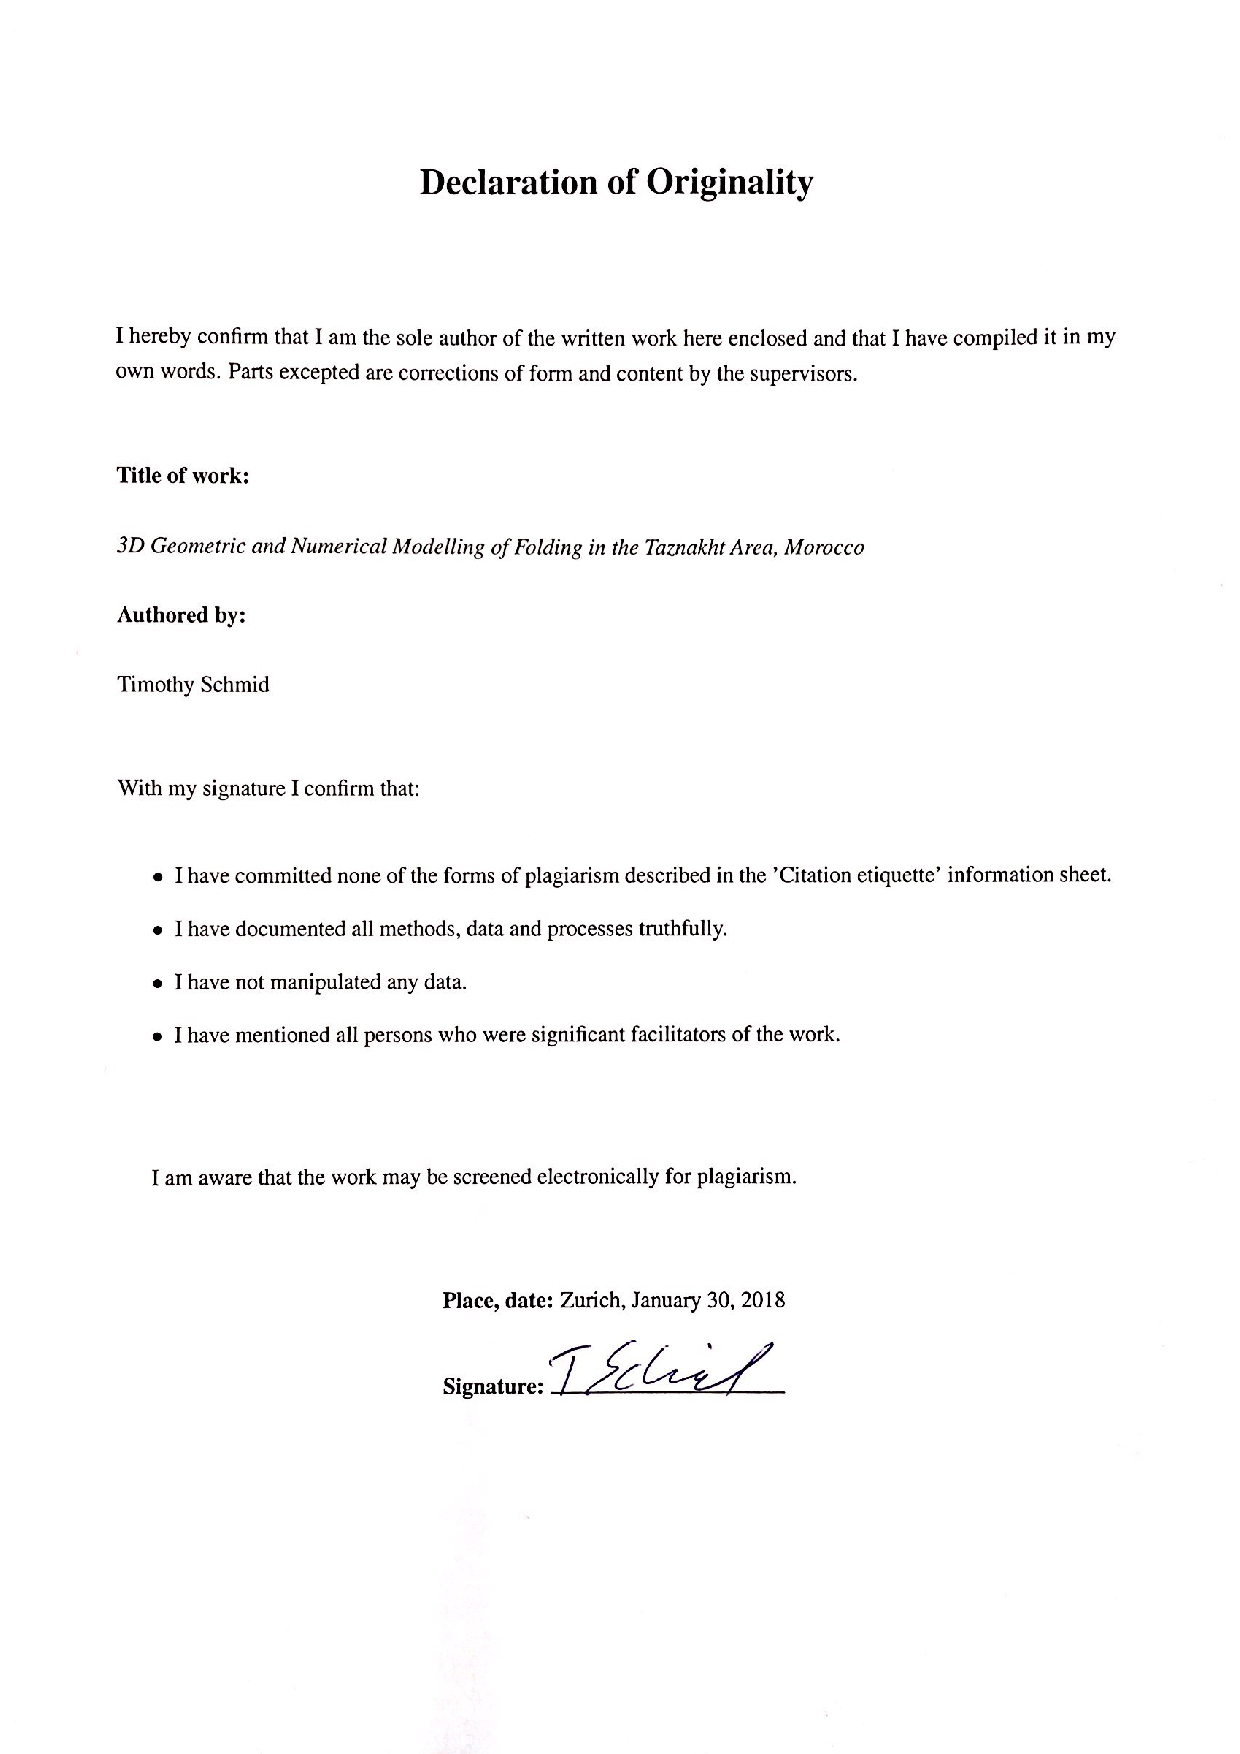
\includepdf[pages={1}]{Declaration.pdf}
%\end{comment}

% ========================================================================== %


% ========================================================================== %
%                                                                            %
%                                 ABSTRACT                                   %
%                                                                            %
% ========================================================================== %



% ========================================================================== %
%                                                                            %
%                              TABLE OF CONTENTS                             %
%                                                                            %
% ========================================================================== %

\newpage
\tableofcontents
\thispagestyle{empty}

\newpage


% ========================================================================== %
%                                                                            %
%                                 INTRODUCTION                               %
%                                                                            %
% ========================================================================== %

\vspace*{10pt}
\section{Introduction}

The Bingham Canyon Open Pit Copper mine houses one one the world's largest Cu-Au-Mo porphyry deposits. It is located about 35 km southwest of Salt Lake city, Utah, USA, in the central Oquirrh Mountain range. The mine has been in use since 1906 and has an annual yield of over 230 kt Cu at an average ore grade of 0.74\%, 12 t Au at 0.4458 g/t, 15kt Mo averaging at 0.035\% and 100 t Ag with 3.29 g/t (Porter et al., 2012; Rio Tinto, 2017 Annual Report).

%
========================================================================== %
%                                                                            %
%                 BACKGROUND AND RESULTS TO DATE         %
%                                                                            %
% ========================================================================== %

\vspace*{10pt}
\section{Background \& Results to Date}

The Bingham Canyon mining district has been thoroughly researched in the past and still is being studied today. Some geochronological studies have been done in this region, which I want to highlight in this section.




% ========================================================================== %
%                                                                            %
%                    			              Goal									  %
%                                                                            %
% ========================================================================== %

\vspace*{10pt}
\section{Goal}

The aim of this study is to determine the ages of the garnet mineralization within the skarn deposits in the Bingham canyon  Cu-Au-Mo porphyry. Multiple geochronology projects have been completed in previous studies for this region, but none have been done for the garnet mineralization within the skarns.

% ========================================================================== %
%                                                                            %
%                 						Geology         							%
%                                                                            %
% ========================================================================== %

\vspace*{10pt}
\section{Geology}

\subsection{Tectonic Setting}
asdaasdasd

% ========================================================================== %
%                                                                            %
%                                 METHODOLOGY                                %
%                                                                            %
% ========================================================================== %

\vspace*{10pt}
\section{Methodology}

\subsection{U/Pb and Sm/Nd radioctive series}
The basis of radiometric dating methods is radioactive decay. This process describes hot an unstable atomic nucleus of an element loses energy and emits radiation and particles, which transforms the parent atom into a daughter nuclide. 

\subsection{Samples}
The samples to be analyzed with the following steps have been gathered by ?? from different locations. The whole rock samples have been derived from the mining district by drilling in three different locations, targeting different areas of the skarn deposits, one near the Au-Cu-rich porphyry stockwerk at the center (Au-Cu center, ACC), one from the Cu-rich peripheral region (Cu-rich periphery, CRP) and one from a deeper, more barren skarn deposit near the core of the stockwerk (Deep Barren Core, DBC). Two boreholes are at the ACC, D652 and D363, four boreholes are located at the CRP, D406, D628, D290 and D077, and the single borehole D794 reaches the DBC. Per borehole one whole rock sample has been extracted and transported to ETH Zürich. Thin sections have been prepared by ?? for further analysis and some thick sections as well. 


\subsection{Petrography}

\subsubsection{Microscopy}

Analysis of minerals & textures from thin sections using polarized light microscopy. Maybe analysis of opaque minerals with reflected light microscopy. Take pictures to determine good microdrilling locations for later garnet extraction.
§

\subsubsection{Microdrilling}

Extraction of select garnet crystals by microdrilling.

\subsection{Chemistry}

\subsubsection{Microprobe Analysis}

Analysis of the thin sections with an electrone micro probe analyzer (EMPA). Non-destructive method to make a highly precise and quantitative element-analysis of the thin sections with high resolution. We can also use this tool do determine the differences in the garnet's cores and zonations.
\\
\noindent For the sample preparation the thin sections must be coated with a layer of graphite, ca. 20nm thick. The voltage is set to ?? kV and therefore determines that the accelerated electrons have ?? keV. The set voltage is also a facilitating factor for the resolution of the result. With higher voltage the resolution would be increased, but the amount of excited elements would decrease and vice versa. 

EDS or WDS mode or both?

\subsubsection{Thermal Ionization Mass Spectrometry (TIMS)}

Maybe?

\subsubsection{Laser Ablation Inductively Coupled Plasma Mass Spectrometry (LA-ICP-MS)}

The Laser Ablation Inductively Coupled Plasma Mass Spectrometer is mostly used for analysis of trace-elements due to the low detection limit of about 10 ppb. For the measurements an internal standard is used and it is crucial to know its exact chemical composition. The previously acquired chemical composition of the garnet from the microprobe analysis will be used to determine the reference material used for this method. Since this is a destructive method, it will be conducted last in the series of methods used. 
\\
\noindent In comparison, LA-ICP-MS is not quite as precise as TIMS measurements
\\
\noindent The LA-ICP-MS system at ETH Zürich is a prototype 193 nm ArF Excimer laser ablation instrument with an ELAN 6100 ICPMS system. It is used for the ablation of the sample is a monochromatic UV laser with a wavelength of 193nm. The size of the aperture, through which the laser is aimed is variable and therefore the diameter of the laser can be adjusted between 15 µm - 120 µm.
\\
\noindent When the laser hits, the surface area of the sample is vaporized into particles, which must be fully ionised, for the mass spectrometer to obtain a signal. The particles are brought into the ICP by a a He-Ar carrier gas mixture. The particles is brought through argon plasma at a temperature of 6000 K, achieved by induction of argon with a copper coil. The particles transit the instrument in a vacuum up to a skimmer cone, which scatters the particles depending on their \( \frac{m}{z} \) ratio. The selected ions converge after passing through an ion lens and reach the mass spectrometer.
\\
\noindent The mass spectrometer consists of a quadrupole and an electron multiplie. The specified ions hit a metal plate of the electron multiplier and electrons are emitted. These then travel further, hit other plates and multiply further to achieve a significant signal.



% ========================================================================== %
%                                                                            %
%                                 TIMEPLAN                                   %
%                                                                            %
% ========================================================================== %

% ========================================================================== %
%                                                                            %
%                          DISCUSSION AND CONCLUSION      %
%                                                                            %
% ========================================================================== %

% ========================================================================== %
%                                                                            %
%                              ACKNOWLEDGMENTS                   %
%                                                                            %
% ========================================================================== %

% ========================================================================== %
%                                                                            %
%                                BIBLIOGRAPHY                             %
%                                                                            %
% ========================================================================== %



% ========================================================================== %

\newpage

% ========================================================================== %
%                                                                            %
%                                  APPENDIX                                  %
%                                                                            %
% ========================================================================== %

\end{document}

% ========================================================================== %
%                                                                            %
%                             DOCUMENT ENDS HERE                             %
%                                                                            %
% ========================================================================== %